%%「論文」,「レター」,「レター(C分冊)」,「技術研究報告」などのテンプレート
%% v3.3 [2020/06/02]

\documentclass[technicalreport]{ieicej}
\usepackage[dvipdfmx]{graphicx,xcolor}
\usepackage{float}
\usepackage[fleqn]{amsmath}
\usepackage{newtxtext}% 英数字フォントの設定を変更しないでください
\usepackage[varg]{newtxmath}% % 英数字フォントの設定を変更しないでください
\usepackage{latexsym}
\usepackage{listings}
\usepackage{xurl}
\usepackage{fancyvrb}
\usepackage{multirow}
\usepackage{array}
\usepackage[section]{placeins} % make sure all fig and table do not go to other sections
\usepackage{stfloats} % somehow avoid the possible blank page by fig or table
% \usepackage[normalem]{ulem}
% \useunder{\uline}{\ul}{}
%\usepackage{amssymb}


\renewcommand{\refname}{References} % To get english reference section heading
\renewcommand{\figurename}{Fig.} % To get english figure heading
\renewcommand{\tablename}{Table} % To get english table heading
\renewcommand\UrlFont{\rmfamily} % Fix url font

\lstset{%
    language={Python},
    basicstyle={\small},%
    identifierstyle={\small},%
    commentstyle={\small\itshape},%
    keywordstyle={\small\bfseries},%
    ndkeywordstyle={\small},%
    stringstyle={\small\ttfamily},
    frame={tb},
    breaklines=true,
    columns=[l]{fullflexible},%
    numbers=left,%
    xrightmargin=0zw,%
    xleftmargin=3zw,%
    numberstyle={\scriptsize},%
    stepnumber=1,
    showstringspaces=false,%
    numbersep=1zw,%
    lineskip=-0.5ex,%
    %moredelim=[is][\underbar]{_}{_},%
    keepspaces=true,%
    %escapechar=\@
}

% \jtitle{タイトル}
% \jsubtitle{}
\etitle{A Study of Product Identification System Using Optical Character Recognition}
% \esubtitle{}
\authorlist{%
 \authorentry[chin-shiji@s.okayama-u.ac.jp]{陳 仕璽}{Shixi Chen}{okayama}
 \authorentry[funabiki@okayama-u.ac.jp]{舩曵 信生}{Nobuo Funabiki}{okayama}
 \authorentry[phvf8tn3@s.okayama-u.ac.jp]{坂上 正規}{Masaki Sakagami}{okayama}
 \authorentry[toshida.takashi@astrolab.co.jp]{土信田 高}{Takashi Toshida}{astrolab}
 \authorentry[suga@astrolab.co.jp]{菅 恒平}{Kohei Suga}{astrolab}
% \authorentry[メールアドレス]{和文著者名}{英文著者名}{所属ラベル}
}
\affiliate[okayama]{}
{Okayama University\hskip1em
Tsushimanaka 3-1-1, Okayama, 700--8530, Japan}
\affiliate[astrolab]{}
{Astrolab \hskip1em
Otemachi 2-6-2, Chiyoda, Tokyo, 100-0004, Japan}
%\affiliate[所属ラベル]{和文勤務先\\ 連絡先住所}{英文勤務先\\ 英文連絡先住所}
\jalcdoi{???????????}% ← このままにしておいてください

\begin{document}
% \begin{jabstract}
% %和文あらまし
% \end{jabstract}
% \begin{jkeyword}
% %和文キーワード
% \end{jkeyword}

\begin{eabstract}
    %background
    Recently, the {\em optical character recognition (OCR)} technology has been remarkably progressed due to the advancements of {\em deep learning techniques}. Besides, smartphones equipped with cameras have broadly spread among people around the world. As a result, the product identification from the product label photo using OCR becomes possible as the quick way to identify the product.
    %problem to be solved
    However, the accuracy of OCR is still not $100\%$. Some characters are incorrectly recognized or missing in the recognition result, which must be considered for use. 
    %contribution
    In this study, we propose a {\em product identification system} applying OCR of the label photo taken by a smart phone. The {\em fuzzy search} is adopted to improve the accuracy by finding the best-matching record in the database for the possibly incorrect key by OCR. Since this search takes inadmissibly long time when the database has a lot of records, we also propose the speedup method by limiting the matching records. 
    %evaluation
    For evaluations, we apply the proposal to $396$ label photos. The results show that the CPU time is $15.241sec$ by the naïve search, and $0.984sec$ by the speedup one that limits the number of matching records into $0.24\%$ of the naïve one, where the record hit rate is slightly reduced from $91.16\%$ to $90.91\%$.
\end{eabstract}

\begin{ekeyword}
product identification, OCR, fuzzy search, regular expression, partial word matching
\end{ekeyword}
\maketitle

%+++++++++++++++++++++++++++++++++++++++++++++++
\section{Introduction}
    %background
    Recently, the {\em optical character recognition (OCR)} technology has been remarkably progressed as the advancements of {\em deep learning techniques}, and resulted in the high recognition rate. Besides, smartphones equipped with cameras have broadly spread among people around the world. As a result, the product identification from the product label photo using OCR becomes possible as the quick way to identify the product.

    %problem to be solved
    However, the character recognition rate of OCR is still not $100\%$. Some characters are incorrectly recognized or missing in the recognition result. Then, if a database is available where the correct characters or strings are stored at the record, the {\em fuzzy search} can be adopted to improve the accuracy by finding the best matching record with the recognition result by OCR. Unfortunately, this search will take inadmissibly long time if the database has a lot of records, because it spends much longer time to process one record. 

    %contribution
    In this study, we propose a {\em product identification system} that applies OCR of the label photo taken by a smart phone. The {\em fuzzy search} is adopted to improve the accuracy by finding the best-matching record in the database for the key string extracted by OCR. However, the fuzzy search takes inadmissibly long time when the database has a lot of records. It calculates the similarity distance between the key data and the stored data in each record. Therefore, we also propose the speedup method by limiting the matching records. 

    %speedup method
    The speedup method limits the matching records with the key that contain a part of the characters in the key. In this paper, the alphanumeric string of the key is divided into two halves, and the records containing either of the half string are extracted from the database. After that, the {\em fuzzy search} is applied to the extracted records only instead of the whole records. 

    %evaluation
    For evaluations, we collect $396$ photos of various product labels and their OCR results, and apply our proposal to them. The application results show that the naïve fuzzy search takes $15.241sec$ for the CPU time achieves $91.16\%$ correct rate. Then, the speedup method drastically reduces the CPU time to $0.984sec$ and slightly decreases the correct rate to $90.91\%$, where the number of matching records becomes 0.24\% of the original. The improvement of the correct rate will be in future studies.

    %contents
    The rest of this paper is organized as follows:

    Section~\ref{sec:preliminary} shows preliminary technologies to this study.

    Section~\ref{sec:proposal} presents the product identification system with the naïve logic.

    Section~\ref{sec:speedup} presents the speedup method for the {\em fuzzy search}.

    Section~\ref{sec:evaluation} shows the evaluation results.

    Finally, Section~\ref{sec:conclusion} concludes this paper with future works.

%+++++++++++++++++++++++++++++++++++++++++++++++
\section{Preliminary}
\label{sec:preliminary}
    In this section, we introduce preliminary technologies to our study in this paper.

    \subsection{Levenshtein Distance}
        The {\em Levenshtein distance} represents the string metric for measuring the difference between two sequences of strings \cite{fuzzywuzzy-guidence}. Informally, the {\em Levenshtein distance} between two words is given by the minimum number of single-character editions by either insertions, deletions, or substitutions that are required to change one word into another one, or the {\em mininum edit distace (MED)} \cite{fuzzywuzzy-guidence}-\cite{levenshtein}.         

        The {\em Levenshtein distance} between two strings $a$ and $b$, $lev(a, b)$, can be calculated recursively by:

        \begin{equation}
                \operatorname{lev}(a, b)=\left\{\begin{array}{ll}
                |a| & \text { if }|b|=0 \\
                |b| & \text { if }|a|=0 \\
                \operatorname{lev}(\operatorname{tail}(a), \operatorname{tail}(b)) & \text { if } a[0]=b[0] \\
                1+\min \left\{\begin{array}{l}
                \operatorname{lev}(\operatorname{tail}(a), b) \\
                \operatorname{lev}(a, \operatorname{tail}(b)) \\
                \operatorname{lev}(\operatorname{tail}(a), \operatorname{tail}(b))
                \end{array}\right. & \text { otherwise. }
                \end{array}\right.
        \end{equation}

        where $|x|$ represents the number of characters in the string $x$, $tail(x)$ is a string of all but the first character of string $x$, and $x[n]$ is the $n$th character of the string $x$, starting with character 0. Due to the recursive procedure, the calculation of the {\em Levenshtein distance} between two strings generally takes much longer time than the simple comparison of them.

    \subsection{FuzzyWuzzy}
        {\em FuzzyWuzzy} is the {\em Python} library to calculate the similarity between two alphanumeric strings or sequences by calculating the {\em Levenshtein distance}, relying on the {\em Difflib} module \cite{fuzzywuzzy}-\cite{fuzzywuzzy-git}. In this paper, we use the {\em simple ratio method} of {\em FuzzyWuzzy} to calculate the similarity between two strings that is described by an integer from 0 to 100. When two strings are exactly the same, the similarity is 100. When a five-character string is examined, the similarity against a string that has one different character is $80$. {\bf Command 1} illustrates the command operation example using {\em FuzzyWuzzy} to two five-character strings where only the fourth one is different.
     
        \begin{center}\bf Command 1\end{center}
        \begin{lstlisting}
>>> from fuzzywuzzy import fuzz
>>> fuzz.ratio("A1532", "A15B2")
80      \end{lstlisting}

    \subsection{Information on Product Label}
        The proposed system identifies the product using the information on the product label. As shown in Figure~\ref{fig:label-exp}, the label usually displays the company name, the product name, the product model number, and the production slot number. Among them, the {\em product model number} is used to identify the product in our system, because it is usually uniquely assigned to each product regardless of different companies. Therefore, the accurate recognition of the {\em product model number} becomes the goal of this study.

        \begin{figure}[t] 
            \begin{center}
            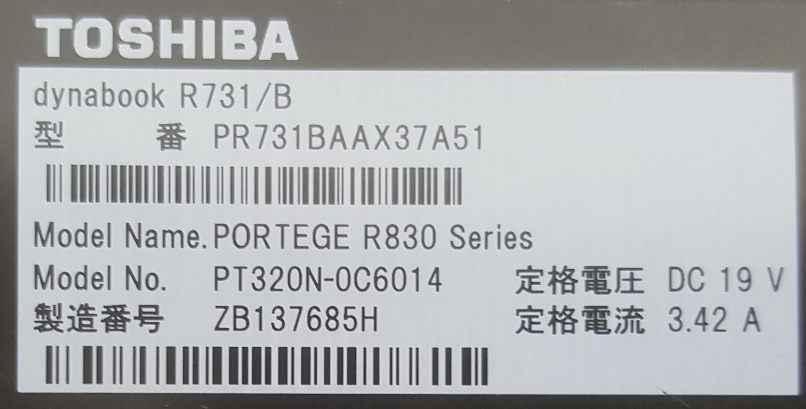
\includegraphics[width=0.48\textwidth]{figure/label-exp.png}
            \end{center}
            \caption{Example product label photo.}
            \label{fig:label-exp}
        \end{figure}


%+++++++++++++++++++++++++++++++++++++++++++++++
\section{Proposal of Product Identification System}
\label{sec:proposal}
    In this section, we propose a {\em product identification system} using OCR and a smartphone camera.
    to fi applying OCR of the label photo taken by a smart phone. The {\em fuzzy search} is adopted to improve the accuracy by finding the best-matching record in the database for the possibly incorrect key by OCR. 

    \subsection{System Overview}
        Figure~\ref{fig:system} illustrates the overview of the proposed product identification system. As the system hardware, a smartphone is used to take a label photo of a target product, to upload the photo to the server, and to display the identification result to the user. Then, a server is adopted to run several programs including the OCR software, the database system, and the product identification program using {\em FuzzyWuzzy}. 

        \begin{figure}[t] 
            \begin{center}
            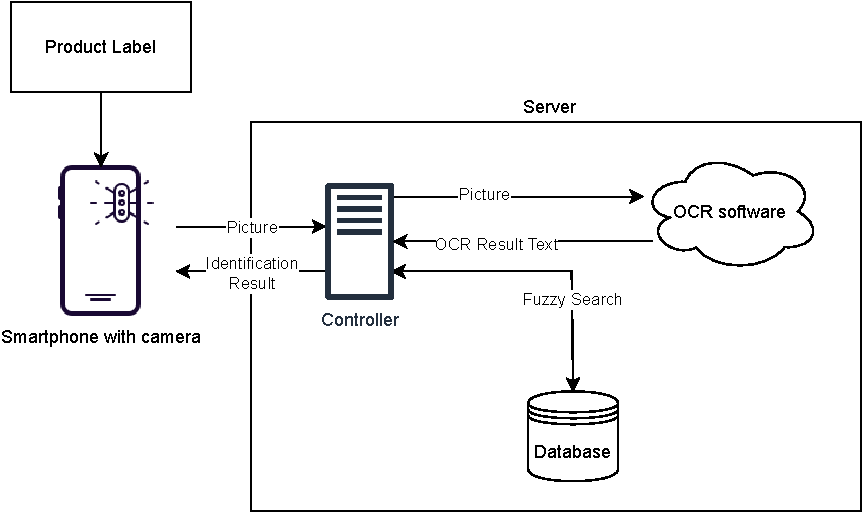
\includegraphics[width=0.48\textwidth]{figure/system.pdf}
            \end{center}
            \caption{System overview.}
            \label{fig:system}
        \end{figure}

    \subsection{System Usage Procedure}
        The usage procedure of the system is described as follows:

        \begin{enumerate}
            \item to take a photo of the product label using a smartphone and upload it to the server using the web browser,
            \item to recognize the characters on the label from the photo using an OCR software on the server,
            \item to extract a set of the candidate strings for the {\em product model number} from the recognized characters by using the {\em regular expression}, 
            \item to calculate the similarity between each candidate string and every records in the database,
            \item to select all the records that have the larger similarity than the given threshold, and display the corresponding product model numbers in descending order of the similarity to the user. 
        \end{enumerate}

        In the following subsections, the details of each step will be explained.

    \subsection{Label Photo by Smarphone}
    \label{sec:label-requirement}
        Open the homepage of this tool, like shown in Figure~\ref{fig:homepage} click the file selection button to take a photo. The camera app of smartphone will be automatically called up.

        \begin{figure}[t] 
            \begin{center}
            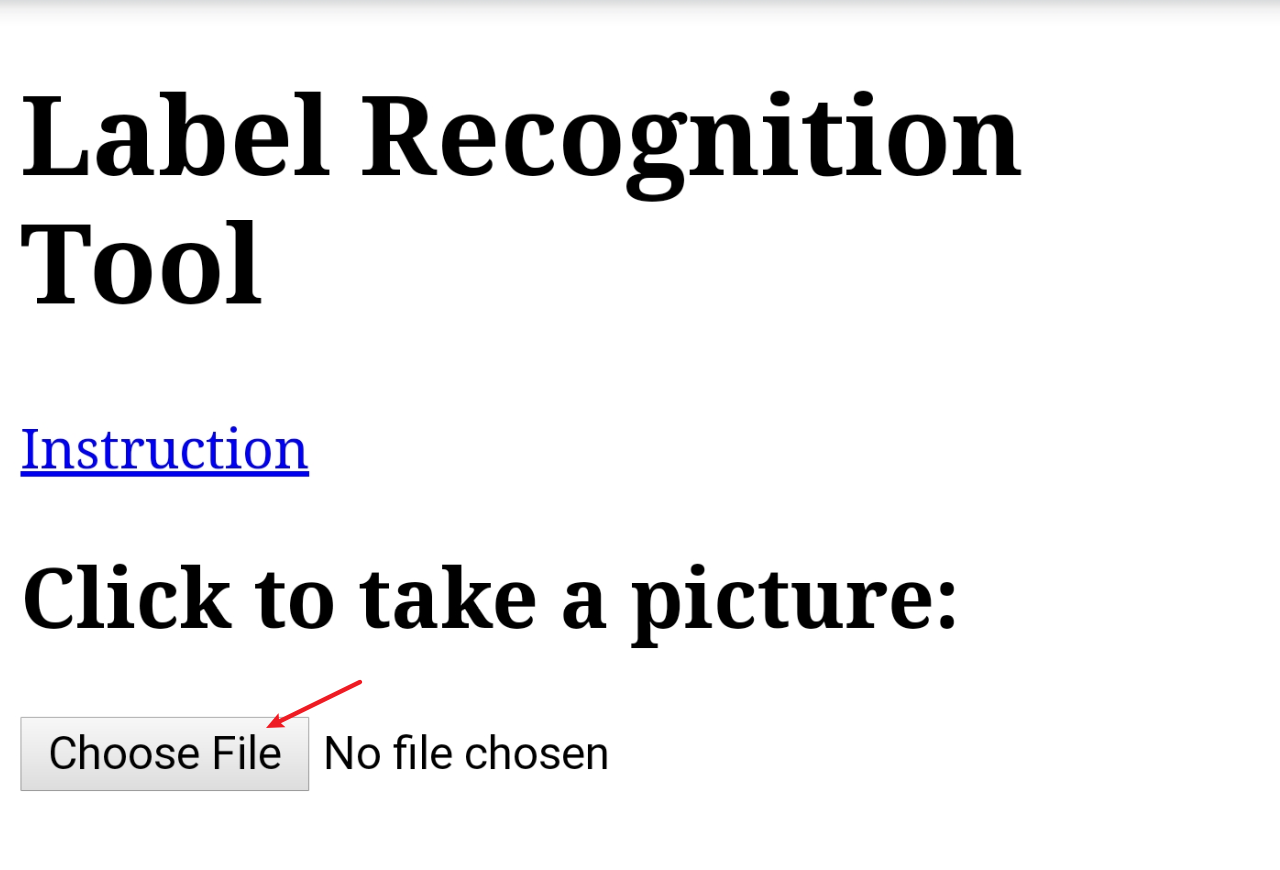
\includegraphics[width=0.48\textwidth]{figure/homepage.png}
            \end{center}
            \caption{Web homepage.}
            \label{fig:homepage}
        \end{figure}

        \begin{figure}[t] 
            \begin{center}
            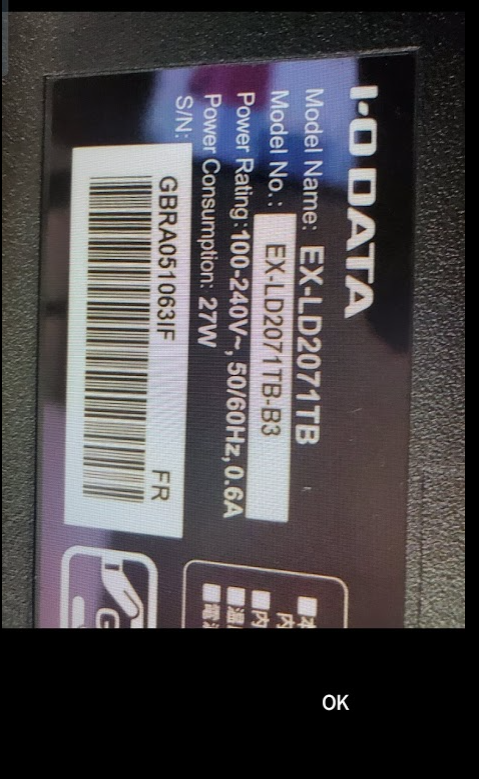
\includegraphics[width=0.48\textwidth]{figure/camera.png}
            \end{center}
            \caption{Take a photo and click OK.}
            \label{fig:camera}
        \end{figure}

        Like shown in Figure~\ref{fig:camera}, use the camera to take a photo and click OK, the browser will then upload the photo to the server. The photo must be taken from the front of the product label. It must ensure that the ambient light is good so that the text on the label is clearly identifiable and try to avoid reflections. As the brightness, contrast, or other environmental condition when the pictures of product labels are taken changes, the accuracy of recognition can fluctuate significantly. The picture should be taken with as few unrelated backgrounds as possible.

    \subsection{Character Recognition by OCR Software}
        On the server, the label photo is input to an OCR software to recognize the characters in the photo.

    \subsection{Candidate Extraction by Regular Expression}
        The following regular expression is used to filter and extract all the alphanumeric strings from the OCR result, as the candidates to the product model number:

            \begin{center}
            \begin{BVerbatim}
[ :]*((?=[a-zA-Z0-9\-\/\(\)]*[0-9])
[a-zA-Z0-9\-\/\(\)]{4,})[ ,.]*
            \end{BVerbatim}
            \end{center}
    
        The {\em [ :]*} in the beginning is set to exclude any possible guiding space or colon before the alphanumeric string we need. Then, in the long expression with the brackets, {\em ((?=[a-zA-Z0-9$\backslash$-$\backslash$/$\backslash$($\backslash$)]*[0-9])[a-zA-Z0-9$\backslash$-$\backslash$/$\backslash$($\backslash$)]\{4,\}) }, the {\em (?=[a-zA-Z0-9$\backslash$-$\backslash$/$\backslash$($\backslash$)]*[0-9])} is called positive look-ahead in the regular expression. It asserts that the following alphanumeric string should be ending with a number\cite{lookahead}-\cite{regex-tutorial}. This positive look-ahead just indicates what the following string should be. However, it does not actually pick any string, so that the string may contain a number in the middle rather than at the end. The following {\em [a-zA-Z0-9$\backslash$-$\backslash$/$\backslash$($\backslash$)]\{4,\})} is the one that actually picks a string more than four characters in length, containing letters, numbers, brackets, hyphen, or slashes, without any space.

        In other words, the alphanumeric string must be more than four characters in the length, by containing letters, numbers, brackets, hyphen, or slashes.

        Finally {\em [ ,.]*} is used to exclude any possible following space, comma, or dot after the alphanumeric string, and make sure the string ends at the correct position.

        
\subsection{Similarity Calculation}
    \label{sec:algorithm.ocrregex}
        If at least one candidate string for the product model number is extracted in the previous step, the similarity between each candidate string and every record in the database is calculated using {\em FuzzyWuzzy}. For this purpose, the database must be prepared in advance to contain the information data for any possible product to be identified in the system. Figure~\ref{fig:db-sample} shows a part of this database. The number of records in this database increases as the number of products to be identified by the system increases.

        \begin{figure}[t]
            \begin{center}
                \begin{tabular}{l|l}
                \Hline
                name & model\_name \\
                \Hline
                CM 690 III & CMS-693-KKN1-JP \\
                EVO Plus & MB-MC128GA \\
                dynabook PC & PT45NWY-SHA \\
                ThinkPad X1 Tablet & 20GH-A06VJP \\
                GALAXY TAB A & SM-T510 \\
                ThinkSystem & ST50 \\
                au & T003 \\
                ideapad S340-14IIL & 81VV \\
                bizhub & 224e \\
                COREFIDO & B820n \\
                ThinkCentre & M900 Small \\
                dynabook & PT45UWP-SWA \\
                Smart-UPS 750 & SUA750JB \\
                PageWide XL & XL 8000 \\                  
                \Hline
                \end{tabular}
            \end{center}
            \caption{Part of database records.}
            \label{fig:db-sample}
        \end{figure}

\subsection{System Output}
    Finally, the system outputs all the product model numbers in the database that have the $70$ or larger similarity in descending order. Since the OCR accuracy is not high enough, our system outputs any possible candidate of the the product model number, and asks the user to choose one manually to improve the accuracy. In most cases the first candidate is the correct one. Figure~\ref{fig:result-sample} shows the output to the label photo in Figure~\ref{fig:camera}. Here, seven candidates for the product model number are displayed, and the first one is correct.

        \begin{figure}[t] 
            \begin{center}
                \begin{BVerbatim}
Matched Model:
{
    "EX-LD2071TB": 100,
    "EX-LDGC271TB": 87,
    "EX-LD2071TNV": 87,
    "EX-LDQ271DB": 82,
    "EX-LDH271DB": 82,
    "100-MR140": 71,
    "100-LA024": 71
}
                \end{BVerbatim}
            \end{center}
            \caption{Sample result list of the system}
            \label{fig:result-sample}
        \end{figure}


%+++++++++++++++++++++++++++++++++++++++++++++++
\section{Proposal of Speedup Method for Fuzzy Search}
\label{sec:speedup}
    In this section, we present the speedup method for the fuzzy search using the partial word matching.

    In the naïve logic, the most time-consuming procedure is {\em Similarity Calculation}. As the similarity between candidate strings and all the records in database have to be calculated. So we add several procedures to limit the range of records from the database, to speedup the calculation.

        \subsection{Half Divided String}
            After \em{Candidate Extraction by Regular Expression}, we divide each extracted candidate alphanumeric string into two halves from the center of the string.

        \subsection{Partial Word Matching}

            For the OCR errors of model text, in most cases, the number of incorrectly recognized characters may not exceed one.

            Thus we divide one alphanumeric string into two halves. For each half, partial matching is performed. Like in table \ref{table:half_matching}. We use partial matching rather than forward or backward matching so that we can avoid OCR text missing.

            In this way, if the misrecognized character is in the second half, the first half is a correct recognition. Partial matching can ensure that the completely matched correct model from the master database is included in the matching result. Conversely, if the misrecognized character is in the first half, partial matching can also help us to match the correct model.
            
            Let the original label text be “MX1234567” and the OCR result be “MX12345b7”, with one error. As shown in table \ref{table:half_matching}, it is divided into “MX123” and “45b7”. The matching result will contain the correct “MX1234567” model and together with some other models sharing the same half with less similarity, then output all of them into the result list.

            \begin{table}[tb]
                \caption{Half divided string and its matching results}
                \label{table:half_matching}
                \begin{center}
                    \begin{tabular}{c|c|c}
                    \Hline
                    origional label text & \multicolumn{2}{c}{MX1234567} \\ 
                    \hline
                    OCR result & \multicolumn{2}{c}{MX12345{\em b}7} \\ 
                    \hline
                    half divided strings & \_\_MX123\_\_ & \_\_45{\em b}7\_\_ \\
                    \hline
                    matching results & \begin{tabular}{c}MX123\underline{4567}\\MX123\underline{5678}\\\underline{P}MX123\underline{5678}\\...\end{tabular} & (no result)) \\
                    \Hline
                    \end{tabular}
                \end{center}
            \end{table}
        
%+++++++++++++++++++++++++++++++++++++++++++++++
\section{Evaluation}
\label{sec:evaluation}
    In this section, we evaluate the proposed system. 

    \subsection{Photo Source}
        We took more than 400 photos to perform the test, and we used 396 of them which match the photo request described in section \ref{sec:label-requirement}.

    \subsection{Regular Expression Used for Matching}

        \begin{figure}[t] 
            \begin{center}
                \begin{BVerbatim}[commandchars=\\\{\}]
NEC
AC ADAPTOR \textcolor{red}{ADP64}
\textcolor{red}{PC-VP-WP36-01/OP-520-75601-01}
\textcolor{red}{ANEC-Y7097Y} N)(S) (D) (FI
D FI
KETI \textcolor{red}{HU10104-2008}
INPUT: AC \textcolor{red}{100-240V 50-60} Hz \textcolor{red}{130-195VA}
OUTPUT: DC 19V 3.16A
S/N(IF ): \textcolor{red}{7919595DA}
MODEL ( O:\textcolor{red}{ADP-60NH}
INPUT (A)(MA):100-\textcolor{red}{240V}~ 1.5A \textcolor{red}{50-60HZ} S
OUTPUT()():19V==3.16A ODO
\textcolor{red}{ADP-60NH}
MARK
NEC Personal Products, Ltd. 0 2 0 85 6 -0 0
                \end{BVerbatim}
            \end{center}
            \caption{An example of regular expression matching result}
            \label{fig:result-regex}
        \end{figure}

        As shown in figure \ref{fig:result-regex}, which is a test result using regex101\cite{regex101}. The red strings are the alphanumeric strings matched. We can see that the correct model {\em ADP-60NH} is among the result. Although the same string is matched multiple times, we can remove the duplicate ones later.

    \subsection{Result}
            
        We conducted 396 searches in a master database with 553,887 records.

        \subsubsection{Regular Expression Matching Rate}

            \begin{table}[t]
                \caption{Regular expression matching result}
                \label{table:regex_result}
                \begin{center}
                    \begin{tabular}{c|c}
                    \Hline
                    Items Tested & 396 \\ 
                    % \hline
                    Correct Model Extracted in Results & 311 \\ 
                    % \hline
                    Correct Model Missed in Results & 85 \\ 
                    % \hline
                    Correct Extracting Rate (\%) & 78.54 \\ 
                    % \hline
                    Average Amount of Strings Extracted for One Item & 8.654 \\ 
                    % \hline
                    Mininum Amount of Strings Extracted for One Item & 1 \\ 
                    % \hline
                    Maximum Amount of Strings Extracted for One Item & 38 \\ 
                    \Hline
                    \end{tabular}
                \end{center}
            \end{table}

            As shown in table \ref{table:regex_result}, among all the tests, in most cases the alphanumeric string containing correct model is successfully extracted by our regular expression. The correct extracting rate is about 78.54\%. There are still 85 cases in which our regular expression failed to match the correct model. But this does not cause an overall failure because we still have fuzzy search to correct minor matching errors.
            
            The average amount of strings extracted for one item is 8.654. All these results will be used as keywords in later fuzzy search. The minimum amount of strings extracted for one item is 1, while the maximum is 38.

        \subsubsection{Speed-up Method for Fuzzy Search Process}

            The time consumed is shown in the table \ref{table:methods_compare}.
    
            \begin{table*}[t]
                \caption{Performance result using different searching methods}
                \label{table:methods_compare}
                \begin{center}
                    \begin{tabular}{c|cc}
                    \Hline
                    search method &
                        \begin{tabular}{c} Conventional Method \end{tabular} &
                        \begin{tabular}{c} Speed-up Method \end{tabular} \\ 
                    \hline
                    Recognized as the 1st candidate in matching list &
                        340 & 339\\ 
                    \hline
                    Recognized in top 5 candidates in matching list &
                        361 & 360\\ 
                    \hline
                    Recognition Rate &
                        91.16\% & 90.91\%\\ 
                    \hline
                    Average Search Time &
                        15.241s & 0.984s \\ 
                    \hline
                    Median Search Time &
                        12.470s & 0.910s \\ 
                    \hline
                    Maximum Search Time &
                        64.273s & 3.004s \\ 
                    \hline
                    Average Search Range (DB Record Amount) &
                        553,887.00 & 1,347.68 \\
                    \Hline
                    \end{tabular}
                \end{center}
            \end{table*}

        \subsubsection{Analyse}

            Using conventional method, there are $340$ cases in which the first candidate in result list is the correct one. In $361$ cases the correct models are among the top $5$ candidates. If we consider matched in the top $5$ candidates as successful recognition, the recognition rate is $91.16\%$. The average searching time for each item is $15.241sec$, median is $12.470sec$, while the maximum is $64.273sec$. As for each item we look up all the records in master DB, the average search range is the amount of records in DB: $553887$.
            
            Using speed-up method, there are $339$ cases in which the first candidate in result list is the correct one. In $360$ cases the correct models are among the top $5$ candidates. If we consider matched in the top $5$ candidates as successful recognition, the recognition rate is $90.91\%$. The average searching time for each item is $0.984sec$, median is $0.910sec$, while the maximum is $3.004sec$. The average search range for each item is $1347.68$, which means the amount of DB record we looked up in fuzzy search.

            \begin{table*}[t]
                \caption{Performance result using different searching methods}
                \label{table:slowest_rec}
                \begin{center}
                    \begin{tabular}{c|c|c|c|c|c|c|c}
                    \Hline
                        \begin{tabular}{c}Real \\Model\end{tabular} &
                        \begin{tabular}{c}Reuglar\\Expression\\Matching Results\end{tabular} &
                        \begin{tabular}{c}Reuglar\\Expression\\Matching Correct\end{tabular} &
                        \begin{tabular}{c}Partial Word\\Matching\\Costed Time (s)\end{tabular} &
                        \begin{tabular}{c}Fuzzy Search\\Total Costed\\Time (s)\end{tabular} &
                        \begin{tabular}{c}Fuzzy Search\\Range (DB\\Record Amount)\end{tabular} &
                        \begin{tabular}{c}Fuzzy\\Search\\1st matched\end{tabular} &
                        \begin{tabular}{c}Fuzzy Search\\top 5\\matched\end{tabular} \\ 
                    \Hline
                    DC35 & 14 & False & 0.26997 & 1.80353 & 24675 & False & False \\ 
                    \hline
                    DM-E25AW & 29 & True & 0.35329 & 2.41260 & 2912 & True & True \\ 
                    \hline
                    TPC-F026-SF & 23 & False & 0.33008 & 2.51139 & 6761 & True & True \\ 
                    \hline
                    K04A-WH & 38 & True & 0.46103 & 2.53164 & 5009 & True & True \\ 
                    \hline
                    MRO-GS8 & 22 & True & 0.31031 & 2.91033 & 3822 & True & True \\ 
                    \hline
                    NE-BS805-K & 33 & True & 0.40080 & 3.00420 & 5574 & True & True \\ 
                    \Hline
                    \end{tabular}
                \end{center}
            \end{table*}

            Among the Fuzzy Search limited by partial word matching results, the several experiments in which the time-consuming is significantly higher than the average time-consuming are as in the table \ref{table:slowest_rec}. We can see the time costed is up to $3.004sec$, with searching ranges of up to $24675$ records.

            
            Using the speed-up method can effectively reduce the time into the acceptable range while increasing the accuracy rate to be close to that of the conventional method. With this method, we can take a balance between searching speed and mistake prevention for OCR text, and successfully limit the search range into over one thousand (about $0.24\%$ of all data amount). In most cases the search result would come out in only less than $2$ seconds which is acceptable for users to wait.
            
            As shown in figure \ref{fig:graph-time} and \ref{fig:graph-recognized}, our speed-up method for fuzzy search is proved to be effective.

            \begin{figure}[t] 
                \begin{center}
                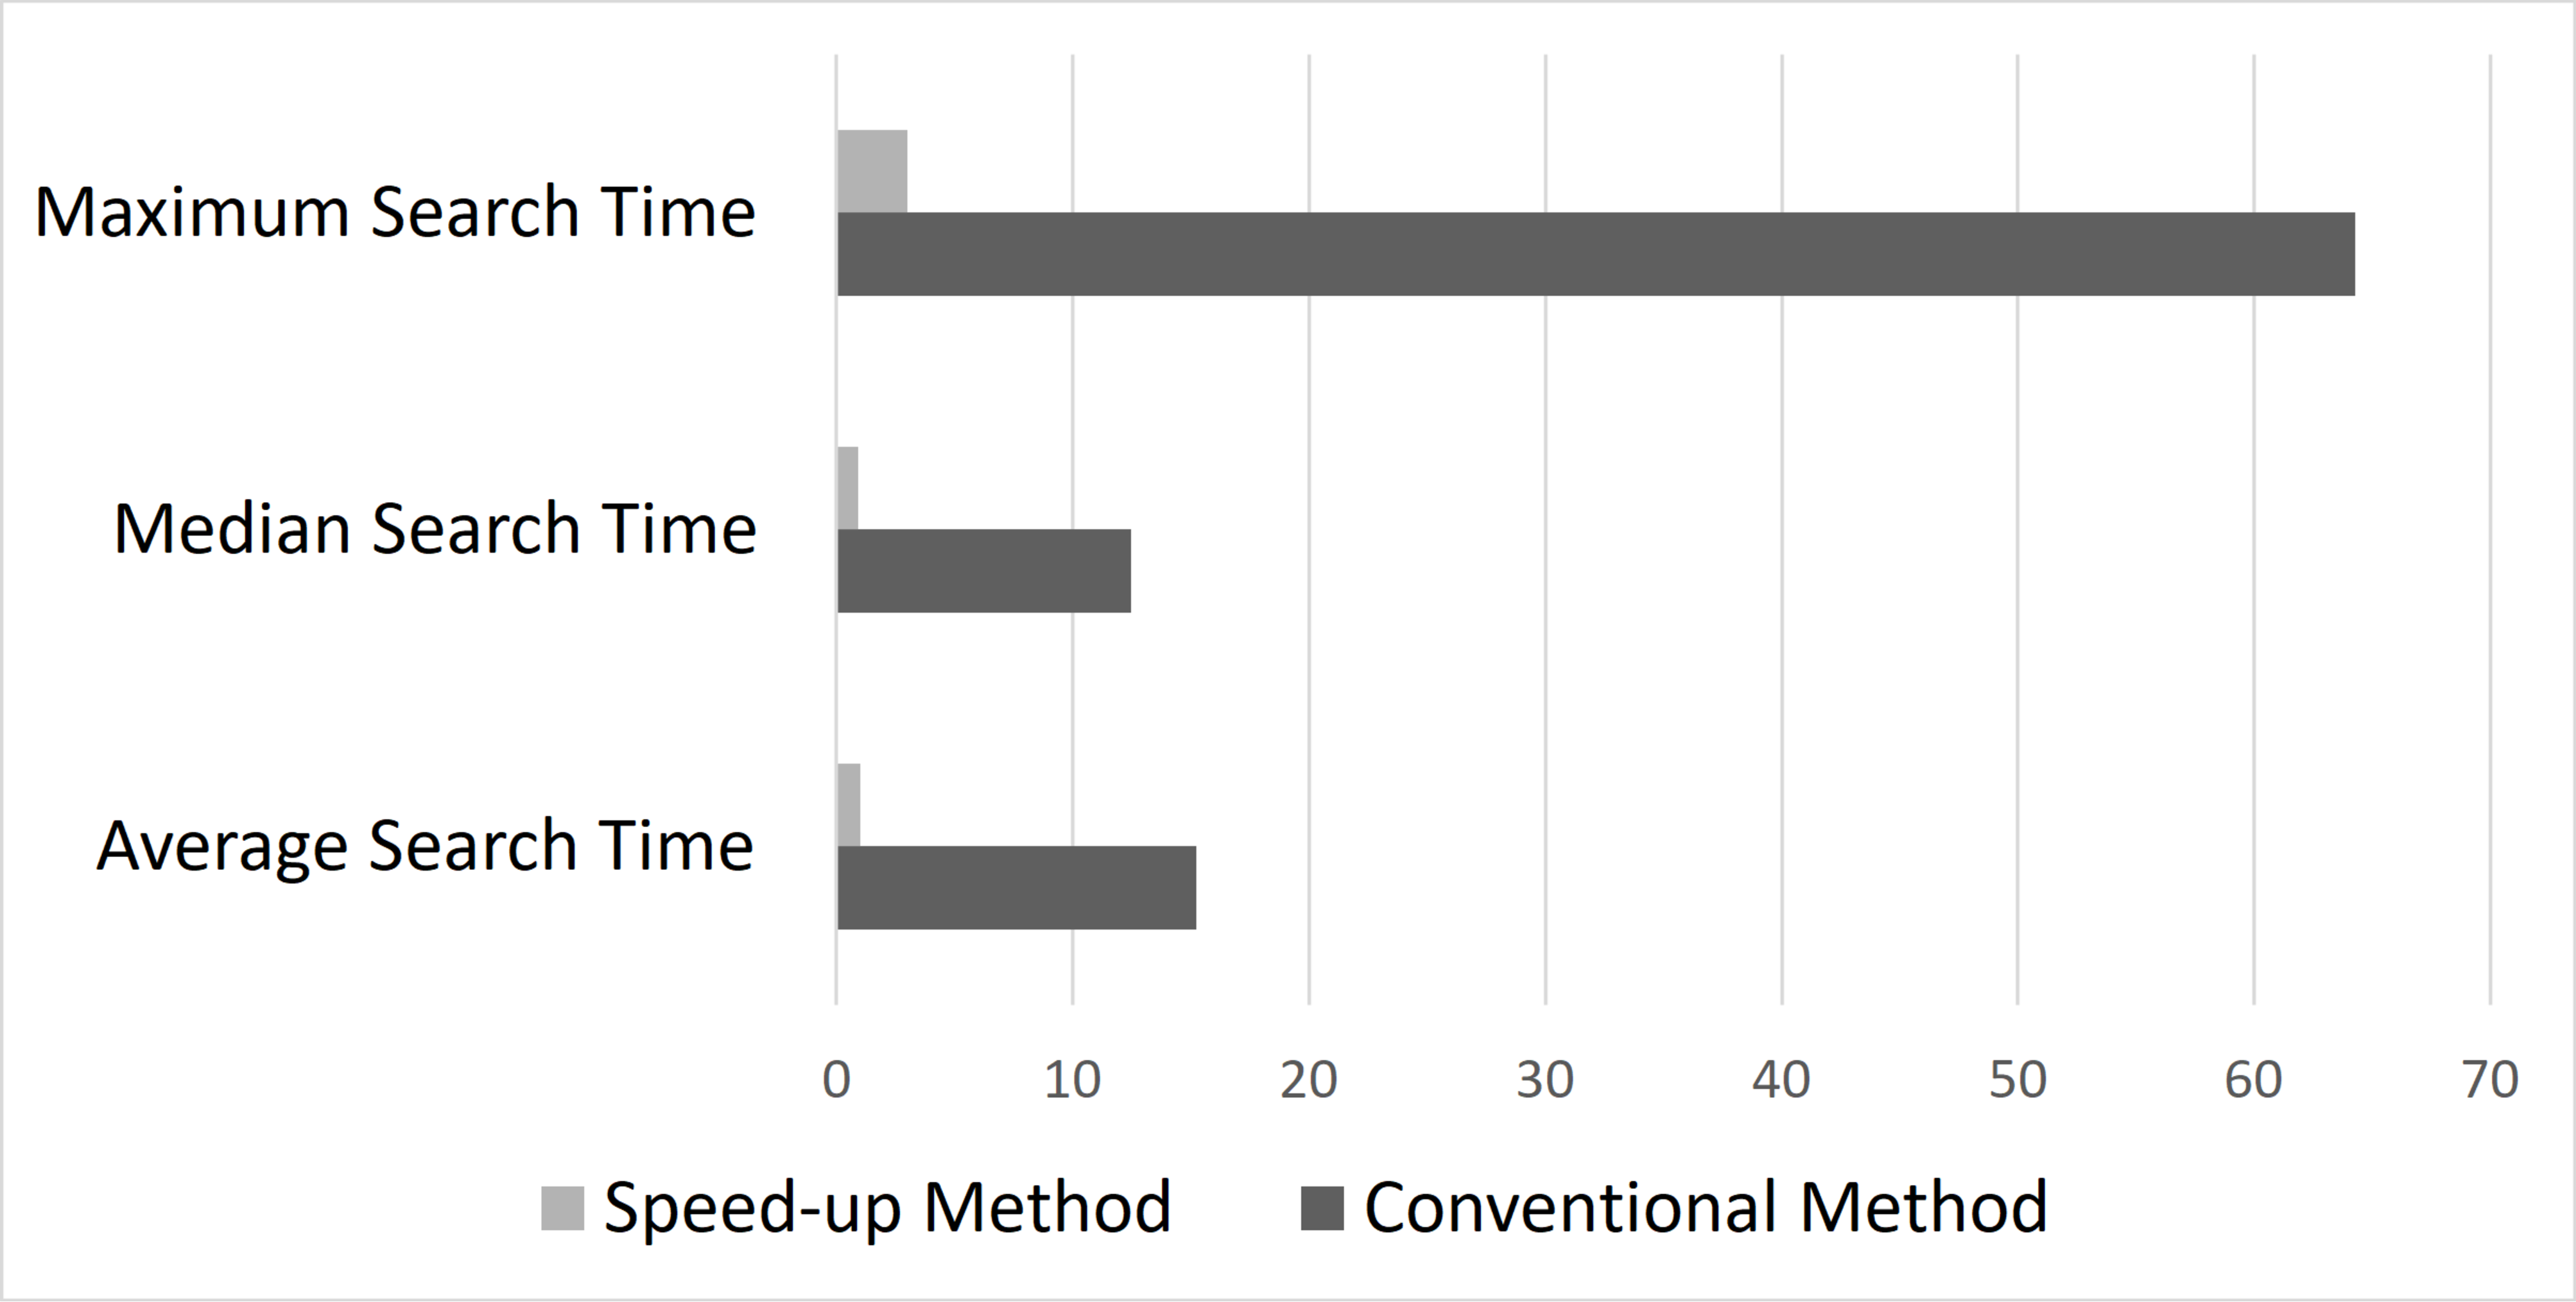
\includegraphics[width=0.48\textwidth]{figure/graph-time.pdf}
                \end{center}
                \caption{Search Time Comparation}
                \label{fig:graph-time}
            \end{figure}

            \begin{figure}[t] 
                \begin{center}
                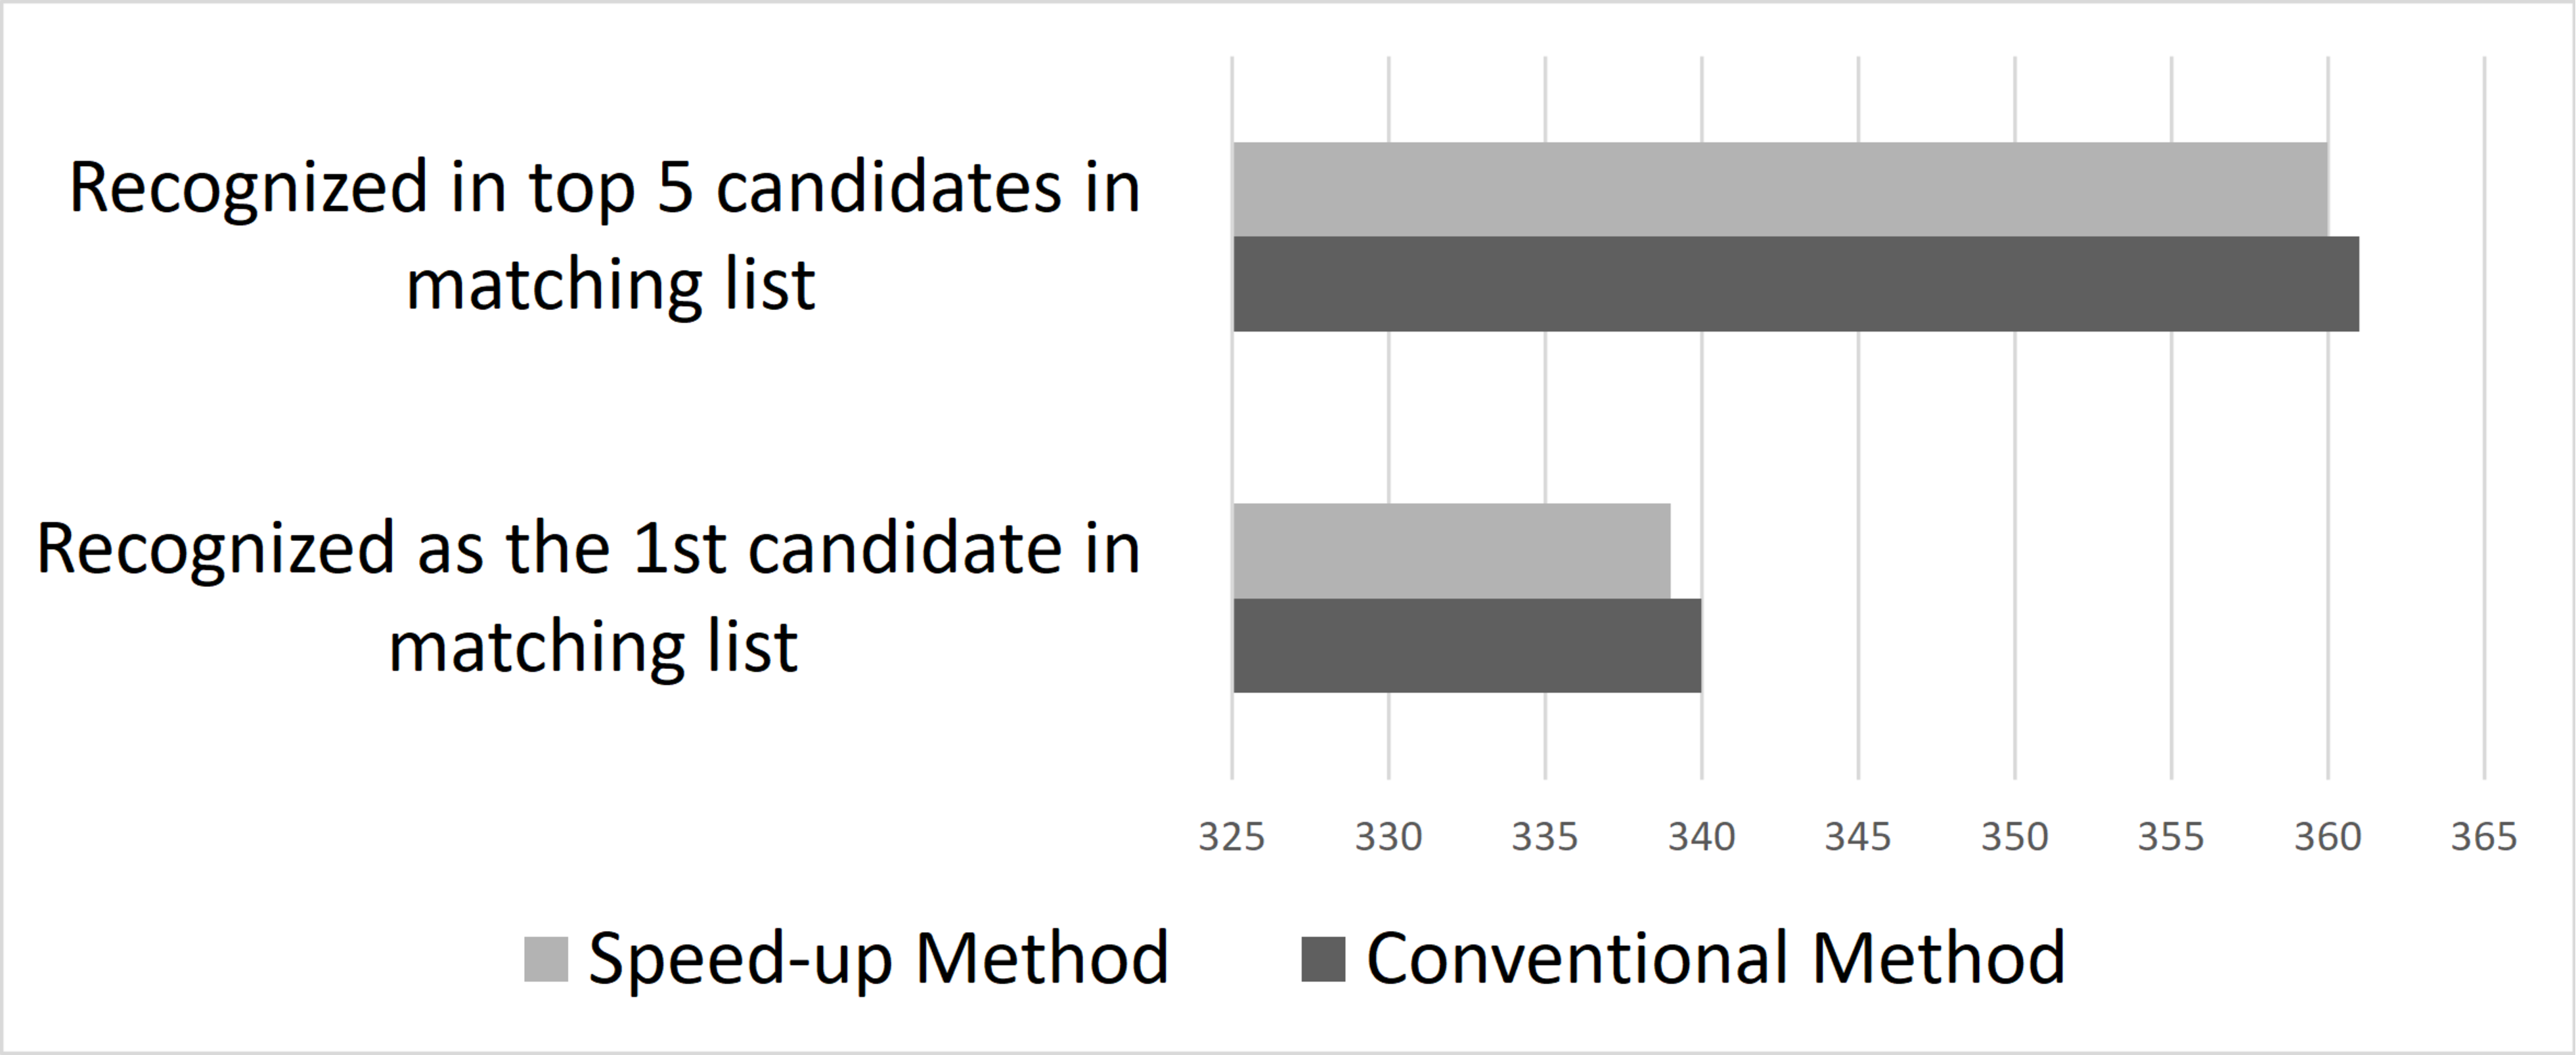
\includegraphics[width=0.48\textwidth]{figure/graph-recognized.pdf}
                \end{center}
                \caption{Search Time Comparation}
                \label{fig:graph-recognized}
            \end{figure}

            
            It can be seen from table \ref{table:slowest_rec} that for few cases, after the limitation of character recognition, the search range is still large, thus it took longer than average time and not as fast as expected. The longest searching time of over $3$ seconds. This indicates that we can still do more to further improve this method.
               
     
%+++++++++++++++++++++++++++++++++++++++++++++++
\section{Conclusion}
\label{sec:conclusion}
    In this section, we conclude this study with future works.

    In this study, we proposed the {\em product identification system} using OCR of the label photo by a smart phone. The {\em fuzzy search} is adopted with the speedup method to improve the accuracy by finding the best-matching record in the database. The application results to $396$ label photos showed the effectiveness of the proposal. In future works, we will improve the user interface and further investigate the performance of the proposal with various product label photos.
            
    We consider that, for each record in the master database, we can add not only the model text information of the product, but also its brand or manufacturer information. Before doing fuzzy search, we can also use other recognition methods to match and analyze the text contained in the OCR results to determine the brand of the product, and use brand information matching to further limit the search range of fuzzy search for model texts, which may further improve searching performance.

    Also, for the result of regular expression shown in figure \ref{fig:result-regex}, we can see some alphanumeric strings unrelated with model also got matched. In future studies we need to find better patterns for regular expression to reduce unnecessary fuzzy searching.

    As our output is a list of most possible models in the product label, it is possible that there are several similar models with the same matching rate. How to correctly pick out the correct one is still to be studied.


%+++++++++++++++++++++++++++++++++++++++++++++++
%\bibliographystyle{sieicej}
%\bibliography{myrefs}
\begin{thebibliography}{99}% 文献数が10未満の時 {9}
    \bibitem{fuzzywuzzy-guidence}
    T., B. (2020, November 14). \emph{FuzzyWuzzy: Fuzzy String Matching in Python, Beginner’s Guide.} Towards Data Science. \url{https://towardsdatascience.com/fuzzywuzzy-fuzzy-string-matching-in-python-beginners-guide-9adc0edf4b35}

    \bibitem{string-correction}
    Wagner, R. A., \& Fischer, M. J. (1974). The String-to-String Correction Problem. \emph{Journal of the ACM, 21(1)}, 168–173. \url{https://doi.org/10.1145/321796.321811}

    \bibitem{guide-to-matching}
    Navarro, G. (2001). A guided tour to approximate string matching. \emph{ACM Computing Surveys, 33(1)}, 31–88. \url{https://doi.org/10.1145/375360.375365}

    \bibitem{levenshtein}
    Wikipedia contributors. (2020, December 15). \emph{Levenshtein distance.} Wikipedia. \url{https://en.wikipedia.org/wiki/Levenshtein_distance}

    \bibitem{fuzzywuzzy}
    Cohen, A. (2011, July 8). \emph{FuzzyWuzzy: Fuzzy String Matching in Python.} ChairNerd. \url{https://chairnerd.seatgeek.com/fuzzywuzzy-fuzzy-string-matching-in-python/}

    \bibitem{fuzzywuzzy-git}
    Seatgeek. (2020, February 14). \emph{FuzzyWuzzy.} GitHub. \url{https://github.com/seatgeek/fuzzywuzzy}

    \bibitem{lookahead}
    Goyvaerts, J. (2020, March 9). \emph{Positive and Negative Lookahead.} Regular-Expressions.info. \url{https://www.regular-expressions.info/lookaround.html}

    \bibitem{lookahead-and-behind}
    BoppreH, hwnd, Trzesniewski, L., Stribiżew, W., \& Ivanova, M.(n.d.). \emph{Regular Expressions - Lookahead and Lookbehind.} SO Documentation. Retrieved December 23, 2020, from \url{https://sodocumentation.net/regex/topic/639/lookahead-and-lookbehind}

    \bibitem{regex-tutorial}
    RegexTutorial.org. (n.d.). \emph{Positive \& Negative Lookahead.} Regex Tutorial. Retrieved December 14, 2020, from \url{https://www.regextutorial.org/positive-and-negative-lookahead-assertions.php}

    \bibitem{regex101}
    Dib, F. (2017, March 31). \emph{Online regex tester and debugger.} Regex101. \url{https://regex101.com/}

\end{thebibliography}

\end{document}


